%\documentclass{beamer}
%\usetheme{Pittsburgh}
\documentclass{scrartcl}

\usepackage[utf8]{inputenc}
\usepackage{default}
\usepackage[procnames]{listings}
\usepackage{graphicx}
%\usepackage[toc,page]{appendix}
\usepackage{caption}
\usepackage{hyperref}
\usepackage{color}
%\usepackage{csvsimple}
\usepackage{float}
\usepackage[T1]{fontenc}



%Bibliogrpahy?
\usepackage{bibentry}
%\nobibliography*
%\bibentry{ }


%Python
\definecolor{keywords}{RGB}{255,0,90}
\definecolor{comments}{RGB}{0,0,113}
\definecolor{red}{RGB}{160,0,0}
\definecolor{green}{RGB}{0,150,0}
\lstset{language=Python,
    basicstyle=\ttfamily\scriptsize,
    keywordstyle=\color{keywords},
    commentstyle=\color{comments},
    stringstyle=\color{red},
    identifierstyle=\color{green},
    breaklines = true,
    columns=fullflexible,
    %Numbering and tabs
    %numbers=left,
    %numberstyle=\tiny\color{gray},
    %stepnumber=2,
    %numbersep=1em,
    tabsize=4,
    showspaces=false,
    showstringspaces=false}

\begin{document}

\title{Scientific Experimentation and Evaluation
}
\subtitle{
Assignment: 3.1}
\author{
  Matin, Maryam \\
  Quignon, Christophe
  %Familyname, Name
}
\date{\today}


\maketitle


\section{Design Report}

\subsection{Calibration Setup}
\paragraph{Description}
Heikkila\cite{heikkila}
Zhang\cite{zhang}

\paragraph{Pitfalls}
\begin{itemize}
\item Lighting conditions can make the pattern indistinguishable
\item The camera frame must not move
\item The calibration pattern may be scaled or even distorted during the printing procedure
\item The calibration pattern must be flat and not curved
\item The background must not contain patterns similar to the calibration pattern
\item When the captured imaged is stored, compression should not distort the calibration pattern
\item The lens has to be clean
\end{itemize}


\subsection{Image estimation}
\paragraph{Number of images}
%Zhang\cite{zhang} stated a method that works with at least two different orientations.

For the testrun, we user 20 images from the camera calibration toolbox that can be downloaded under \href{http://www.vision.caltech.edu/bouguetj/calib_doc/htmls/calib_example.zip}{vision.caltech.edu/bouguetj/calib/\_doc/htmls/calib\_example.zip}

\paragraph{Image positions}
%Either the image or the camera can be freely moved and the movement need not be known. (Zhang\cite{zhang}).
%We start with an orthogonal view and then two rotations with roughly 30 $^\circ $ on every axis of the frame.


\subsection{Parameter description}
\begin{itemize}
\item
\begin{lstlisting}[language=Python]
chessdim = (12, 13)
\end{lstlisting}
The dimensionality of the chessboard is given as the number of inside corners
\item
\begin{lstlisting}[language=Python]
criteria = (cv2.TERM_CRITERIA_EPS + cv2.TERM_CRITERIA_MAX_ITER, 30, 0.001)
\end{lstlisting}
We stop the algorithms either after 30 iterations or if an accuracy of 0.001 is met.
Description
\end{itemize}

\paragraph{Code}
(See calibration.py)
\lstinputlisting[language=Python]{calibration.py}

\paragraph{Output}

\paragraph{Parameter description}
%what do they mean

%TODO: insert real values


\begin{itemize}
\item
\begin{lstlisting}[language=Python]
fc = 671.13759, 680.77186]
\end{lstlisting}
Focal length

\item
\begin{lstlisting}[language=Python]
cc = [319.5, 239.5]
\end{lstlisting}
Principal point

\item
\begin{lstlisting}[language=Python]
alpha_c = [0.0] => angle of pixel  = 90.0 degrees
\end{lstlisting}
Skew

\item
\begin{lstlisting}[language=Python]
kc = [0.0, 0.0, 0.0, 0.0, 0.0]
\end{lstlisting}
Distortion

\item
\begin{lstlisting}[language=Python]
err = [0.45330, 0.38916]
\end{lstlisting}
Pixel error


%\item Parameter\\
%Meaning
\end{itemize}


\subsection{Possible Problems}
\paragraph{Calibration}
%Error sources


\begin{figure}[H]
\centering
\begin{minipage}{.5\textwidth}
  \centering
  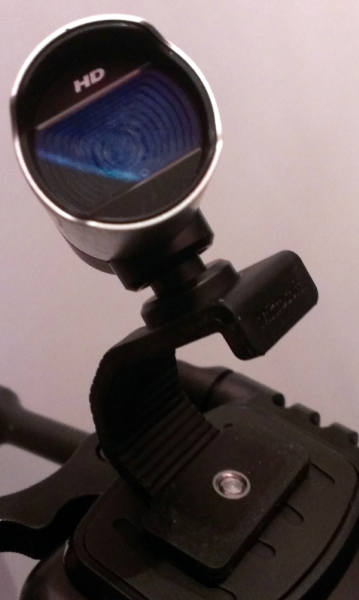
\includegraphics[width=.8\linewidth]{img/rotation.jpg}
  %\caption{}
  %\label{fig:}
\end{minipage}%
\begin{minipage}{.5\textwidth}
  \centering
  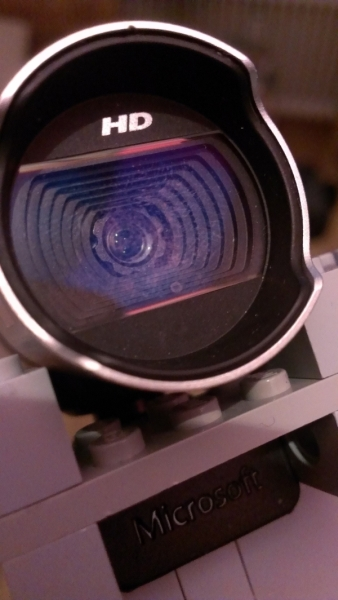
\includegraphics[width=.8\linewidth]{img/lense.jpg}
  %\caption{}
  %\label{fig:} 
\end{minipage}
\caption{Rotation on the tripod (left) and a dirty aperture (right) are source of possible errors.}
\label{fig:errorsources}
\end{figure}
%Description

\begin{figure}[H]
\centering
\begin{minipage}{.5\textwidth}
  \centering
  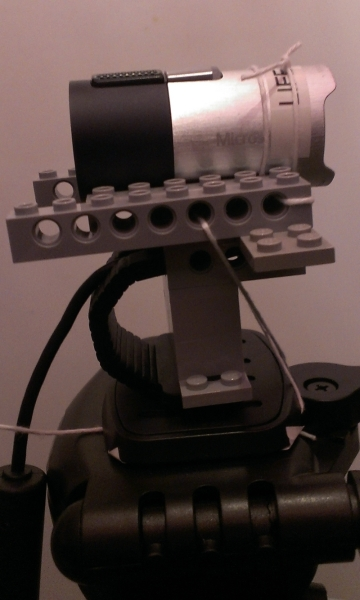
\includegraphics[width=.47\linewidth]{img/fixation_1.jpg}
  %\caption{}
  %\label{fig:}
\end{minipage}%
\begin{minipage}{.5\textwidth}
  \centering
  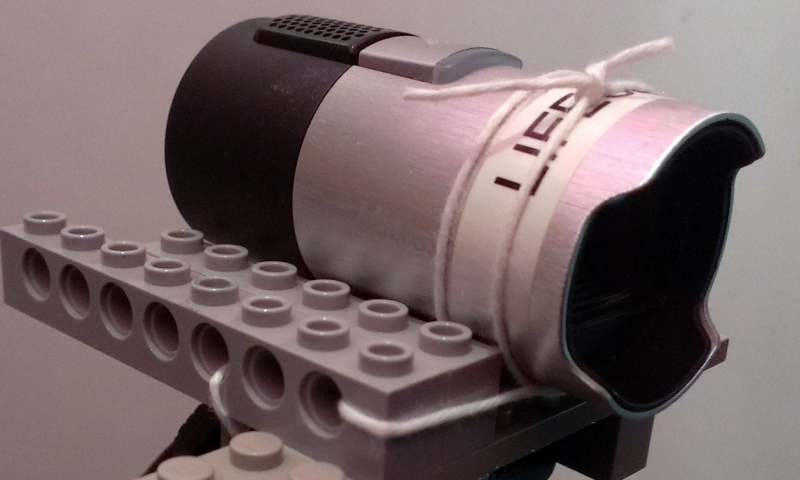
\includegraphics[width=1.3\linewidth]{img/fixation_2.jpg}
  %\caption{}
  %\label{fig:} 
\end{minipage}
\caption{The camera was fixed to the tripod to avoid displacements.}
\label{fig:fixation}
\end{figure}
%Description




\paragraph{Experiment}
%problems while testing including problems with laptop/camera

%The camera connected without any issues
%It is important to release the camera after taking an image, otherwise it will stay blocked
%One has to make sure which index to use, because the index destinguished between the built-in camera of the laptop and the usb camera
%The camera is very light sensitive. It works best at low light.


\begin{figure}[H]
\centering
\begin{minipage}{.5\textwidth}
  \centering
  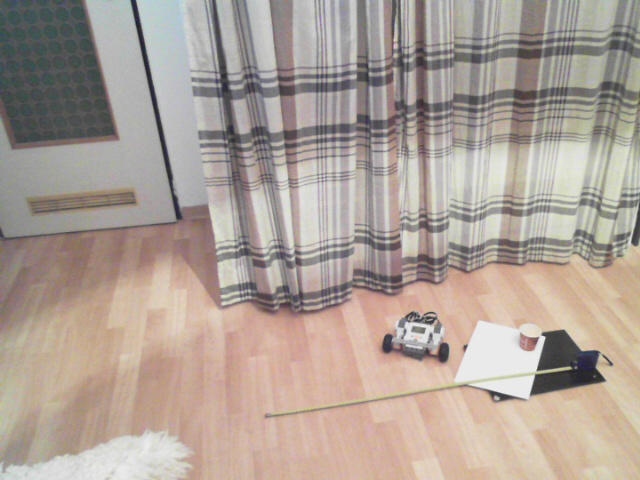
\includegraphics[width=.8\linewidth]{img/testimgbad.jpg}
  %\caption{}
  %\label{fig:}
\end{minipage}%
\begin{minipage}{.5\textwidth}
  \centering
  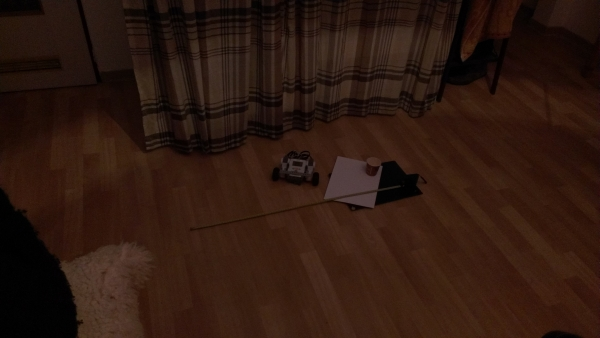
\includegraphics[width=.8\linewidth]{img/iso400.jpg}
  %\caption{}
  %\label{fig:} 
\end{minipage}
\caption{The camera is very light sensitive (left) in comparison to digital ISO 400 (right). In both images the background could disturb the calibration pattern.}
\label{fig:brightness}
\end{figure}
%Description



%maybe we exclude this
\section{Appendix}


\subsection{Code}
(See cam2jpg.py)
\lstinputlisting[language=Python]{cam2jpg.py}

\subsection{Output}


%BIBLIOGRPAHY!
\bibliographystyle{plain}%amsalpha
\bibliography{bib.bib}
%\bibentry{}


%COPY AND PASTE FROM HERE

%\begin{enumerate}
% \item
%\end{enumerate}

%\href{link}{text}

%\begin[Language=Python]{lstlisting}
%#PYTHON CODE HERE
%\end{lstlisting}

%\lstinputlisting[language=Java]{ }

%\csvautotabular[separator=semicolon]{data.csv}

%\begin{figure}
% \center
% \includegraphics[width= cm]{img/ }
% \caption{}
%\end{figure}



\end{document}
